\documentclass[otchet]{SCWorks}
% Тип обучения (одно из значений):
%    bachelor   - бакалавриат (по умолчанию)
%    spec       - специальность
%    master     - магистратура
% Форма обучения (одно из значений):
%    och        - очное (по умолчанию)
%    zaoch      - заочное
% Тип работы (одно из значений):
%    coursework - курсовая работа (по умолчанию)
%    referat    - реферат
%  * otchet     - универсальный отчет
%  * nirjournal - журнал НИР
%  * digital    - итоговая работа для цифровой кафдры
%    diploma    - дипломная работа
%    pract      - отчет о научно-исследовательской работе
%    autoref    - автореферат выпускной работы
%    assignment - задание на выпускную квалификационную работу
%    review     - отзыв руководителя
%    critique   - рецензия на выпускную работу
% Включение шрифта
%    times      - включение шрифта Times New Roman (если установлен)
%                 по умолчанию выключен
\usepackage[T2A]{fontenc}
\usepackage[utf8]{inputenc}
\usepackage{graphicx}
\usepackage[sort,compress]{cite}
\usepackage{amsmath}
\usepackage{amssymb}
\usepackage{amsthm}
\usepackage{fancyvrb}
\usepackage{longtable}
\usepackage{array}
\usepackage[english,russian]{babel}
\usepackage{minted}
\usepackage{tempora}
\usepackage[hidelinks]{hyperref}


\usepackage{multirow}
\usepackage[table]{xcolor}\usepackage{longtable}\usepackage{array}
\usepackage{graphicx}%Вставка картинок правильная

\usepackage{float}%"Плавающие" картинки

\usepackage{wrapfig}%Обтекание фигур (таблиц, картинок и прочего)
\setlength{\arrayrulewidth}{0.5mm}
\setlength{\tabcolsep}{18pt}

\newenvironment{centeritemize*}[1][]
  {\par\centering\begin{itemize*}[itemjoin=\quad,#1]}
  {\end{itemize*}\par}
\newcolumntype{C}[1]{>{\centering\let\newline\\\arraybackslash\hspace{0pt}}m{#1}}


\begin{document}

% Кафедра (в родительном падеже)
\chair{математической кибернетики и компьютерных наук}

% Тема работы
\title{Определение скорости звука в воздухе методом интерференции}

% Курс
\course{1}

% Группа
\group{151}

% Факультет (в родительном падеже) (по умолчанию "факультета КНиИТ")
% \department{факультета КНиИТ}

% Специальность/направление код - наименование
% \napravlenie{02.03.02 "--- Фундаментальная информатика и информационные технологии}
% \napravlenie{02.03.01 "--- Математическое обеспечение и администрирование информационных систем}
% \napravlenie{09.03.01 "--- Информатика и вычислительная техника}
\napravlenie{09.03.04 "--- Программная инженерия}
% \napravlenie{10.05.01 "--- Компьютерная безопасность}

% Для студентки. Для работы студента следующая команда не нужна.
\studenttitle{Студентов}

% Фамилия, имя, отчество в родительном падеже
\author{Григорьева Данилы Евгеньевича и Лазаревой Виктории Владимировны}

% Заведующий кафедрой 
\chtitle{доцент, к.\,ф.-м.\,н.}
\chname{С.\,В.\,Миронов}

% Руководитель ДПП ПП для цифровой кафедры (перекрывает заведующего кафедры)
% \chpretitle{
%     заведующий кафедрой математических основ информатики и олимпиадного\\
%     программирования на базе МАОУ <<Ф"=Т лицей №1>>
% }
% \chtitle{г. Саратов, к.\,ф.-м.\,н., доцент}
% \chname{Кондратова\, Ю.\,Н.}

% Научный руководитель (для реферата преподаватель проверяющий работу)
\satitle{доцент, к.\,ф.-м.\,н.} %должность, степень, звание
\saname{О.\,А.\,Черкассова}

% Руководитель практики от организации (руководитель для цифровой кафедры)
\patitle{доцент, к.\,ф.-м.\,н.}
\paname{С.\,В.\,Миронов}

% Руководитель НИР
\nirtitle{доцент, к.\,п.\,н.} % степень, звание
\nirname{В.\,А.\,Векслер}

% Семестр (только для практики, для остальных типов работ не используется)
\term{2}

% Наименование практики (только для практики, для остальных типов работ не
% используется)
\practtype{учебная}

% Продолжительность практики (количество недель) (только для практики, для
% остальных типов работ не используется)
\duration{2}

% Даты начала и окончания практики (только для практики, для остальных типов
% работ не используется)
\practStart{01.07.2022}
\practFinish{13.01.2023}

% Год выполнения отчета
\date{2023}

\maketitle

% Включение нумерации рисунков, формул и таблиц по разделам (по умолчанию -
% нумерация сквозная) (допускается оба вида нумерации)
\secNumbering

\tableofcontents

% Раздел "Обозначения и сокращения". Может отсутствовать в работе
% \abbreviations
% \begin{description}
%     \item ... "--- ...
%     \item ... "--- ...
% \end{description}

% Раздел "Определения". Может отсутствовать в работе
% \definitions

% Раздел "Определения, обозначения и сокращения". Может отсутствовать в работе.
% Если присутствует, то заменяет собой разделы "Обозначения и сокращения" и
% "Определения"
% \defabbr

\newpage

\begin{enumerate}[leftmargin=3.5cm]
    \item[\bf Наименование работы.] Определение скорости звука в воздухе методом интерференции.
    \item[\bf Цель.] Изучение процесса распространения звуковой волны в газе и измерение скорости звука при различных случаях интерференции волн.
    \item[\bf Принадлежности.] Прибор Квинке, звуковой генератор.
    \item[\bf Рабочая формула.] $v = 4a_1 \nu, v = \frac 4 3 a_2 \nu, v = \frac 4 5 a_3 \nu$
    \item[\bf Ход работы.] Результаты вычислений представлены в таблице.


% После введения — серии \section, \subsection и т.д.
    {\renewcommand{\arraystretch}{1.5}
    \setlength{\tabcolsep}{5pt}
    \rowcolors{3}{black!10!white!50}{black!2!white!90}
        \begin{longtable}[h!]{ |C{1.5cm}|c|C{2cm}|c|c|c|c|c|c|c| }
            \hline
            {№ опыта} & $\nu$, Гц & № мини-мума & $a$, см & $v$, м/c & $\overline v$, м/с & $|\Delta v|$, м/с & $|\overline{\Delta v}|$, м/с & $v_0$, м/c \\
            \hline
            \endhead
            1 & 1200 & 1 & 6,90 & 331,20 & 330,13 & 1,07 & 13,56 & 317,64 \\
            2 & 1200 & 2 & 20,50 & 328,00 & 330,13 & 2,13 & 10,36 & 317,64 \\
            3 & 1200 & 3 & 34,50 & 331,20 & 330,13 & 1,07 & 13,56 & 317,64 \\
            4 & 1500 & 1 & 5,50 & 330,00 & 334,00 & 4,00 & 8,64 & 321,36 \\
            5 & 1500 & 2 & 16,80 & 336,00 & 334,00 & 2,00 & 14,64 & 321,36 \\
            6 & 1500 & 3 & 28,00 & 336,00 & 334,00 & 2,00 & 14,64 & 321,36 \\
            7 & 1800 & 1 & 4,50 & 324,00 & 334,32 & 0,32 & 2,33 & 321,67 \\
            8 & 1800 & 2 & 14,00 & 336,00 & 334,32 & 1,68 & 14,33 & 321,67 \\
            9 & 1800 & 3 & 23,40 & 336,96 & 334,32 & 2,64 & 15,29 & 321,67 \\
            \hline
        \end{longtable}}

$\overline{v_0} \approx 320,22\,\text{м}/\text{с}$ \\
Относительная погрешность составляет $4,57\%$. \\
Максимальная погрешность составляет $6,4\%$

\end{enumerate}


\section*{Выводы}
В результате поставленных опытов с помощью прибора Квинке и звукового генератора методом интерференции (наложения когерентных волн) была вычислена скорость звука в пределах вычисленной ранее абсолютной погрешности.
Подытожим опыт проведенного эксперимента: прибор Квинке наглядно показывает несовершенства слуха и открывает умение находить скорость звука посредством метода интерференции. Нельзя не отметить важность умения находить волны в состоянии резонанса, открытие простейших знаний по работе с лабораторными приборами, подкреплённых практикой. В результате поставленных опытов была вычислена скорость звука в пределах вычисленной ранее абсолютной погрешности.

\section{Контрольные вопросы}

\subsection{Как происходит процесс распространения звука в газе?}
Элементы среды, примыкающие к истоинику колебаний, смещаются из своих положений равновесия и совершают такие же колебания. Смещение происходит в направлении, перпендикулярном к плоскости источника колебаний. Благодаря упругим взаимодействиям между отдельными элементами среды в колебательное движение придут через определённое время и более удалённые элементы. В результате смещений элементов газовой среды их их положений равновесия будут чередоваться области с повышенной и пониженной плотностью по сравнению с той, которая была до прихода волны. Соответственно будет изменяться и давление газа. Колебания с частотой от 16 до 20 000 Гц называются звуковыми.
\subsection{Какими параметрами характеризуется волна? Как распределяется плотность воздуха вдоль трубки в данный момент времени?}
Запишите уравнение плоской бегущей волны. Какими параметрами характеризуется волна? Нарисуйте графики зависимости $\xi = f(x)$ при $t = const$ и $\xi = f(t)$ при $x = const$. Как распределяется плотность воздуха вдоль трубки в данный момент времени? \\
\\
\begin{equation*}
    \xi = A\sin{\omega(t-t_1)} = A\sin{\omega(t-\frac x v)}\text{, где}
\end{equation*}
\begin{itemize}
    \item $\xi$ -- смещение
    \item $A$ -- амплитудное значение смещения
    \item $\omega$ -- круговая частота, определяющая число колебаний за $2\pi$ с
    \item $\omega t$ -- фаза колебания, определяющаlipsumя смещение в данный момент $t$
\end{itemize}
\newpage
График зависимости $\xi = f(x)$ при $t = const$:
\begin{figure}[h!]
    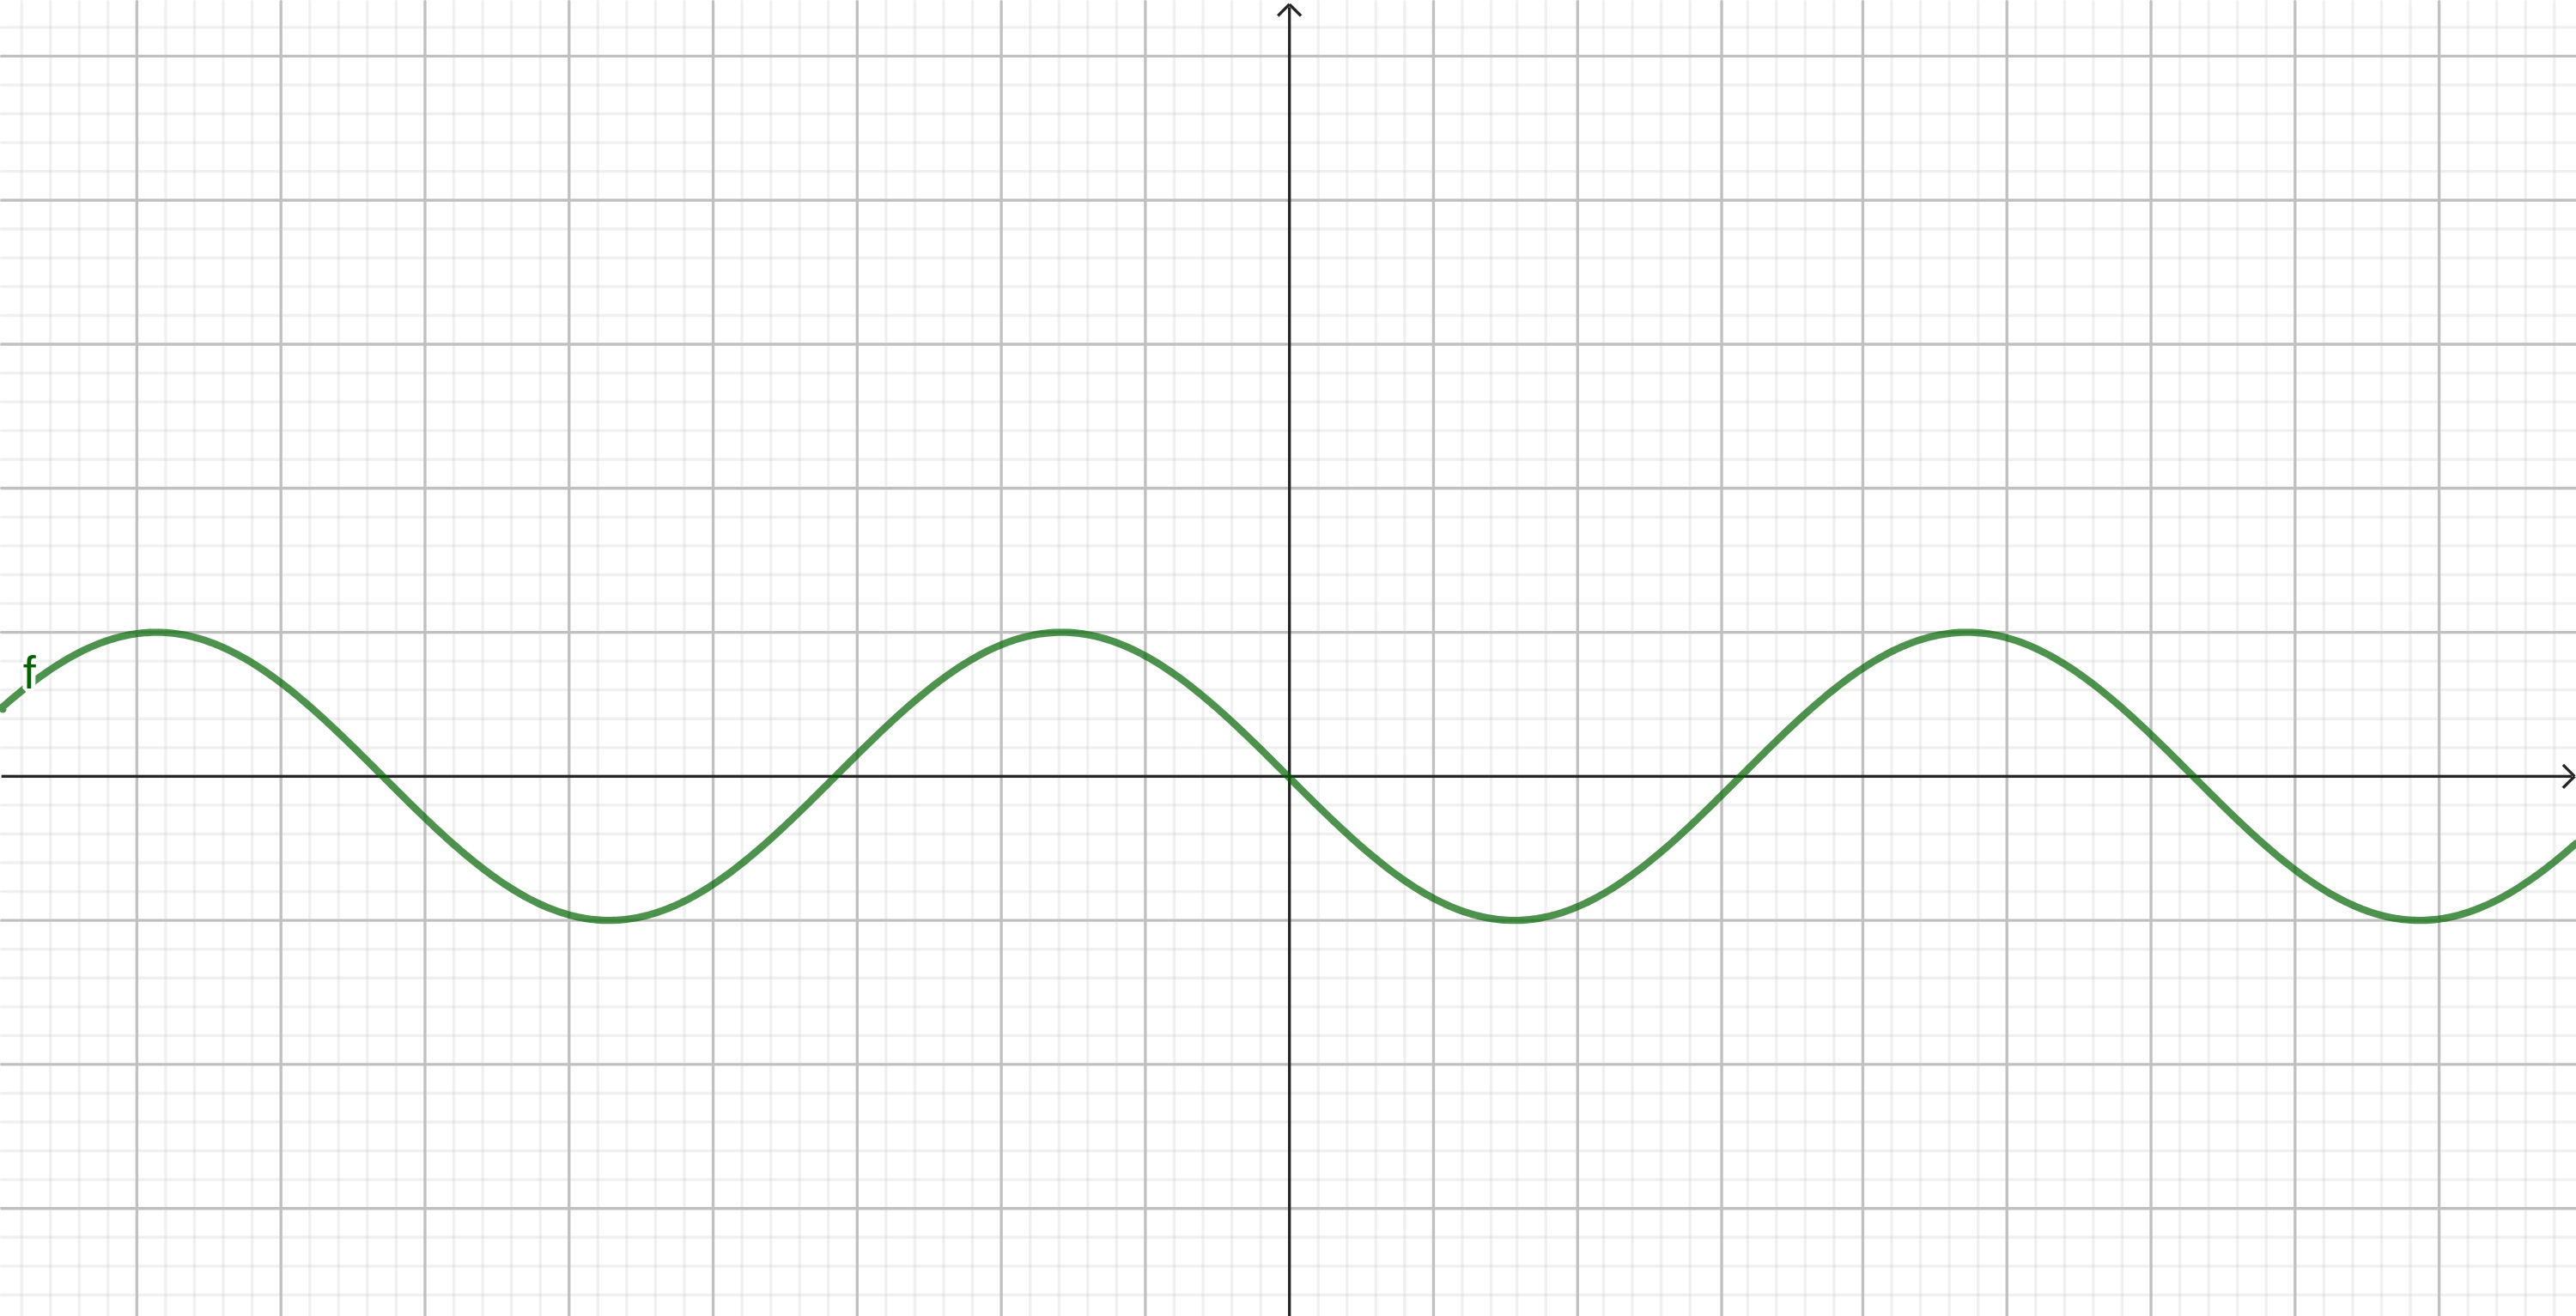
\includegraphics[width=\textwidth]{240312_physics_13.1_1.png}
\end{figure}

График зависимости $\xi = f(t)$ при $x = const$:
\begin{figure}[h!]
    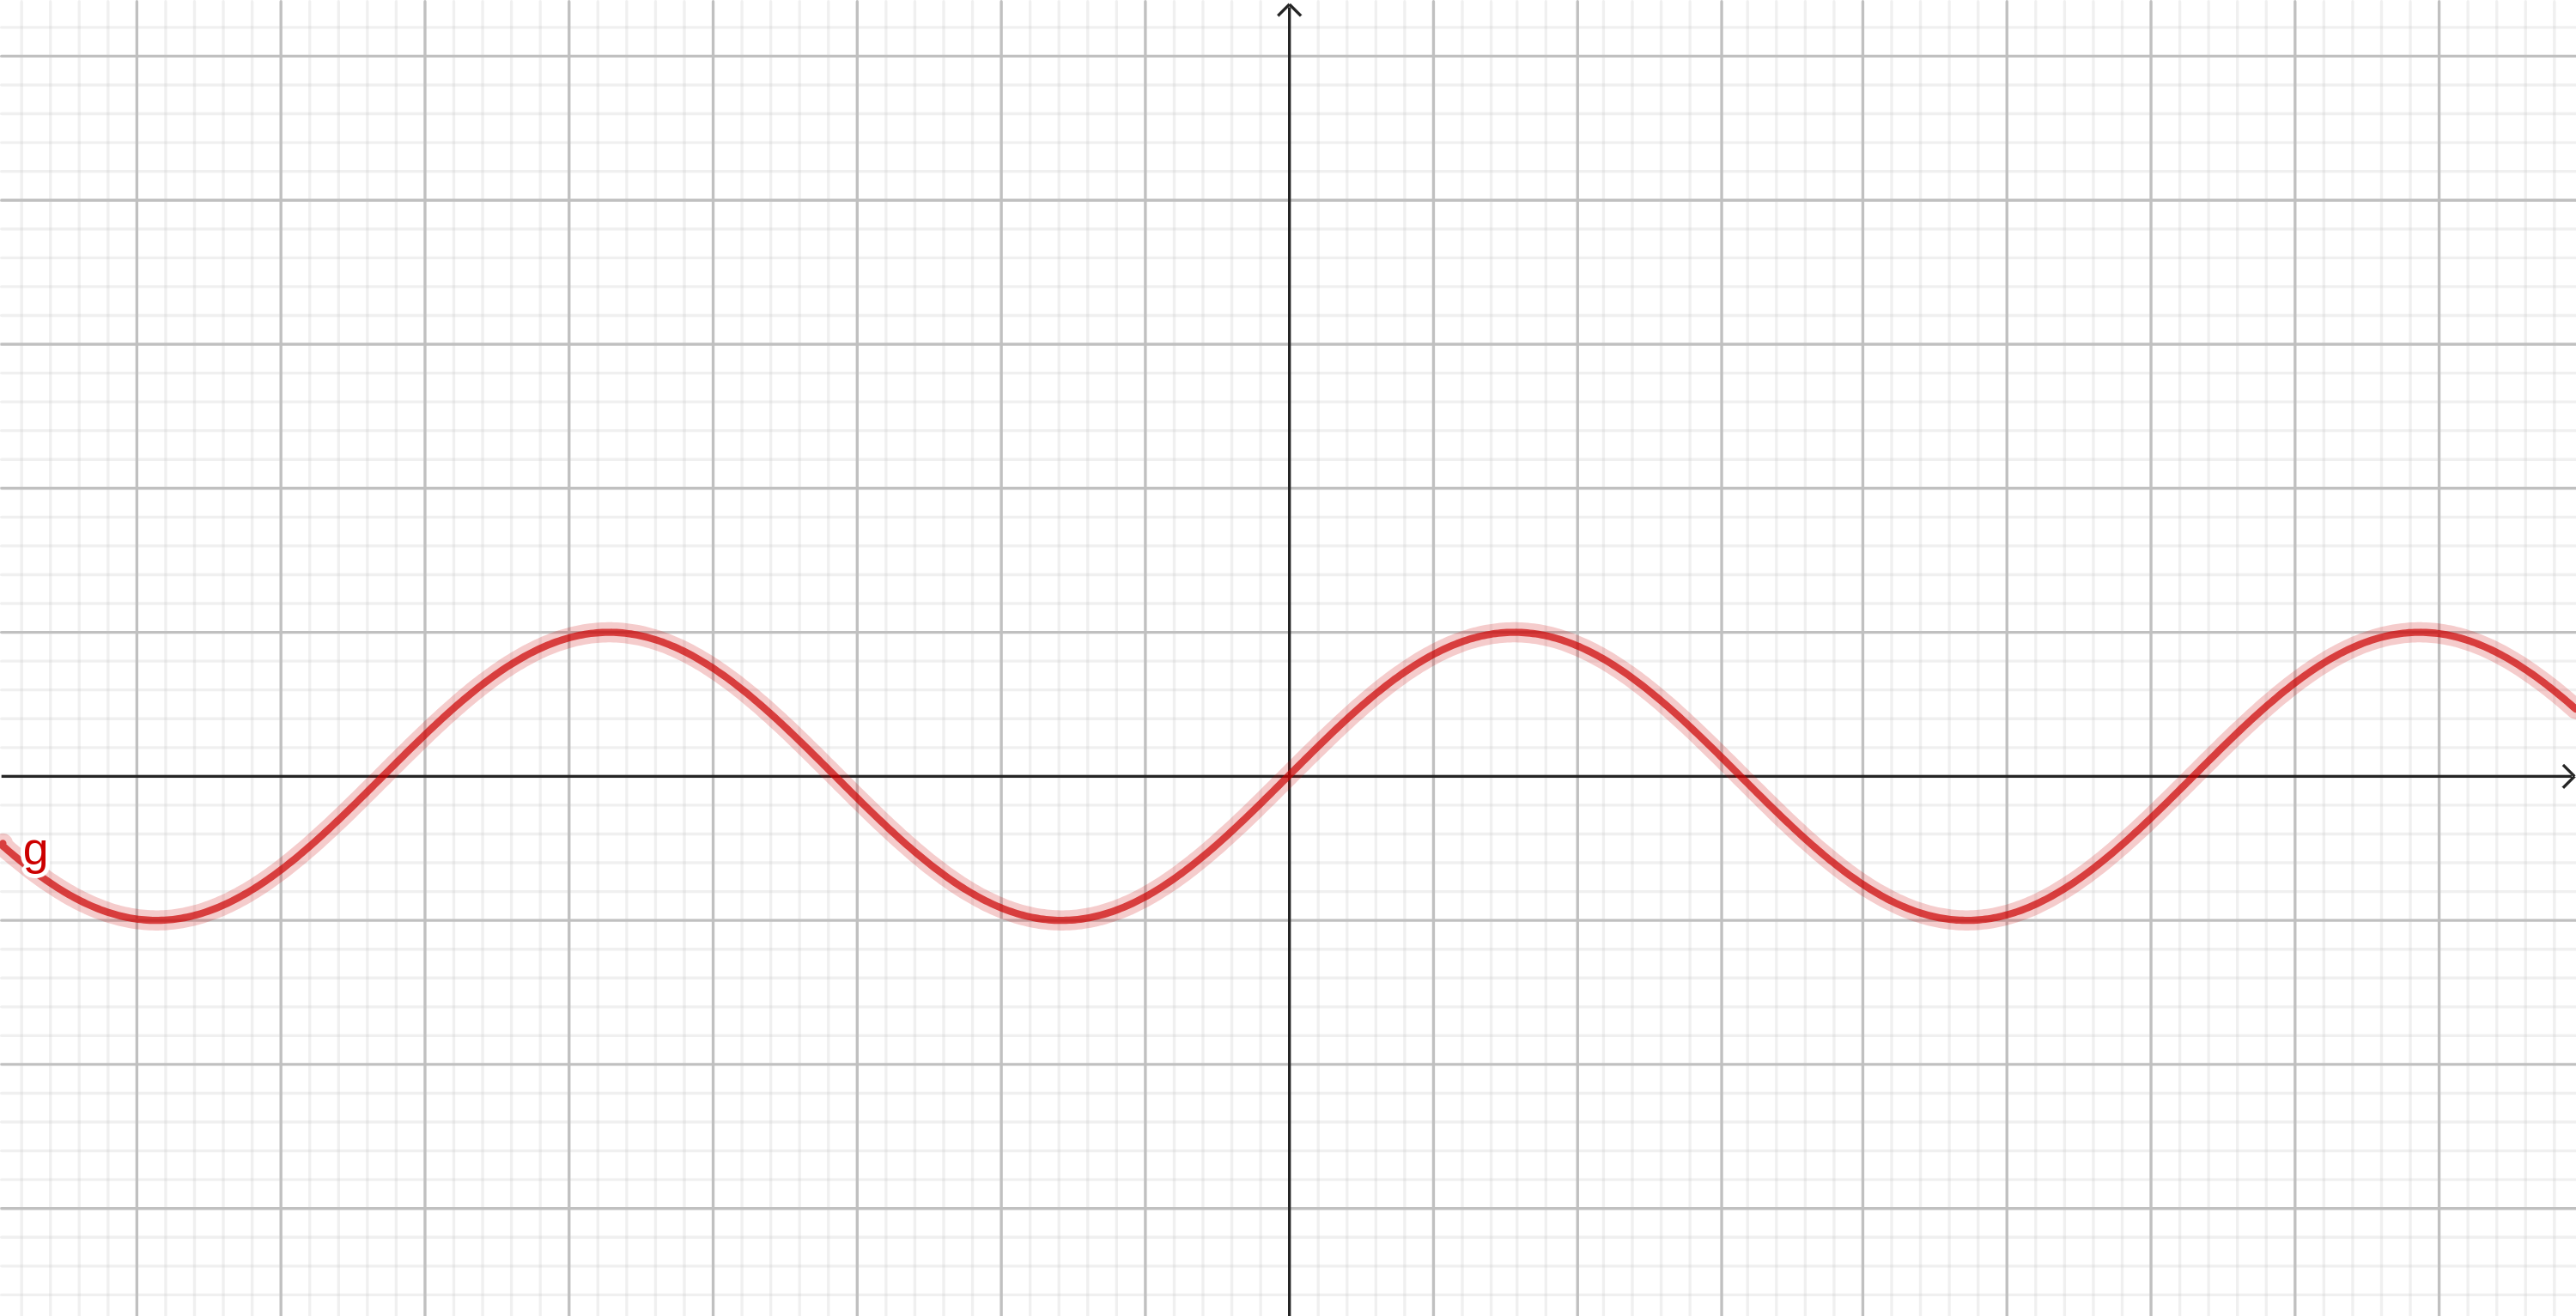
\includegraphics[width=\textwidth]{240312_physics_13.1_2.png}
\end{figure}

\subsection{Как распределятся плотность воздуха вдоль трубки?}
Запишите уравнение стоячей волны. Нарисуйте графики зависимости $\xi=f(x)$ при $t=const$ и $\xi=f(t)$ при $x = const$. Как распределяется плотность воздуха вдоль трубки? \\
\\
В результате смещений элементов газовой среды(воздуха в рассматриваемом опыте) из их положений равновесия вдоль трубки будут чередоваться области с пониженной и повышенной плотностью по сравнению с той, которая в трубке до прихода волны. Отсюда следует, что изменяется давление газа. \\
Если мембрана прибора Квинке колеблется с частотой в диапазоне от 16 до 20000 Гц, то такие колебания плотности газовой среды воспринимаются человеческим ухом(называются звуковыми колебаниями).
\subsection{Как скорость звука зависит от температуры?}
Скорость звука в газах существенно зависит от температуры среды:
\begin{equation*}
    v_0 = \frac{v}{\sqrt{1 + \alpha t}}\text{, где}
\end{equation*}
\begin{itemize}
    \item $v$ -- скорость звука при температуре $t^\circ C$
    \item $t$ -- температура
    \item $\alpha$ -- коэффициент расширения газа ($0,004^{-\circ}$)
    \item $v_0$ -- скорость звука при температуре $0^\circ C$
\end{itemize}

\subsection{В чём заключается явление интерференции волн? Как амплитуда результирующей волны зависит от разности хода интерферирующих волн?}
Интерференция звуковых волн заключается в том, что наложение друг на друга двух волн, имеющих одинаковую частоту, приводит к усилению или ослаблению звуковых колебаний в зависимости от точки пространства. Амплитуда результирующей волны определяется по следующей формуле:
\begin{equation*}
    A^2 = A^2_1 + A^2_2 + 2A_1A_2\cos{2\pi\frac{\Delta x}{\lambda}}\text{, где}
\end{equation*}
\begin{itemize}
    \item $A_1$, $A_2$ -- амплитуды исходных волн
    \item $\Delta x$ -- разность хода
    \item $\lambda$ -- длина волны
\end{itemize}
\subsection{При каких условиях в минимуме интенсивность звуковых колебаний имеет конечное значение?}

\subsection{Как устроена экспериментальная установка для определения скорости звука в воздухе методом интерференции?}
Мембрана телефона создаёт звуковую волну с нужной частотой. Тройник разветвляет звуковую волну на две части, благодаря чему теперь уже две конгерентные волны проходят по двум разным трубкам, длина которых может увеличиваться или уменьшаться. После прохождения волн по трубкам, они соединяются на следующем тройнике, и результирующую волну мы сможем услышать в слуховой трубке.
\subsection{Как устроена экспериментальная установка для определения скорости звука в воздухе методом стоячей волны?}
Основной элемент конструкции - стеклянная трубка, на конце которой находится телефон, который создаёт звуковую волну с необходимой частотой. С помощью слуховой трубке, связанной со стеклянной трубкой через её отросток и резиновый шланг, фиксируется громкость звука. Внутри трубки находится поршень, положение которого определяется с помощью миллиметровой шкалы.


% \conclusion

% Библиографический список, составленный вручную, без использования BibTeX
%
% \begin{thebibliography}{99}
%   \bibitem{Ione} Источник 1.
%   \bibitem{Itwo} Источник 2
% \end{thebibliography}

% Отобразить все источники. Даже те, на которые нет ссылок.
% \nocite{*}

% Меняем inputencoding на лету, чтобы работать с библиографией в кодировке
% `cp1251', в то время как остальной документ находится в кодировке `utf8'
% Credit: Никита Рыданов
\inputencoding{cp1251}
% \bibliographystyle{gost780uv}
% \bibliography{thesis}
\inputencoding{utf8}

% При использовании biblatex вместо bibtex
% \printbibliography

% Окончание основного документа и начало приложений Каждая последующая секция
% документа будет являться приложением
\appendix

\end{document}
